% This bring summarise and bring together all the previous section into a specification that should be fully expanded in the appendix with the following points, in providing what is known as the System Requirements Specification (SRS). This collects various information that you have previously agreed and worked on such as the UML diagrams.
{
\setstretch{1.5}
\section{Purpose}
The main goal of this concept is to provide users a solution to indoor museum navigation through an exciting, and enjoyable experience using augmented reality. It includes users being lost, or searching for a specific location within the museum. It was discovered through field research that the concept would make life easier for users and the museums since it would allow easy access to the information based on exhibitions.

\section{Scope}
This project will include creating an AR application for people to get an enjoyable journey in the museum. The project will be completed by 29 April 2019. The AR application will include simple navigation system to direct various part of the museum. Getting information on the user screen using the user's camera, and explore various museum using the system. The platform will be developed on Android due to the high usage of Google's AR library, ARCore.

\section{System Overview}
The application will perform all the basic tasks to help users with their journey in the museum. Such as navigating from point A to B, getting the user back on track in case they are lost, allowing the user to view information based on camera recognition of an exhibit.

\section{References}
This specification should be read in conjunction with the following publications:\\
IEEE 24765-2017 - ISO/IEC/IEEE International Standard - Systems and software engineering--Vocabulary \cite{IEEE24765}\\
IEEE Std 29148-2011, ISO/IEC/IEEE International Standard - Systems and software engineering -- Life cycle processes --Requirements engineering \cite{IEEE29148} \\
IEEE Std 730-2014, IEEE Standard for Software Quality Assurance Processes \cite{IEEE730} \\
IEEE Std 24748-4-2016 - ISO/IEC/IEEE International Standard for Systems and Software Engineering -- Life Cycle Management -- Part 4: Systems Engineering Planning \cite{IEEE24748}

\section{Definitions}
\textbf{Activity:} A set of cohesive tasks of a process, which transforms inputs into outputs. [ISO/IEC/IEEE 12207:2008]\\
\newline
\textbf{Augmented reality:} A technology that superimposes a computer-generated image on a user's view of the real world, thus providing a composite view. \\
\newline
\textbf{Functional requirement:} A requirement that specifies a function that a system or system component must perform. [ISO/IEC/IEEE 24765:2010]\\
\newline
\textbf{Non-functional requirement:} The measurable criterion that identifies a quality attribute of a function or how well a functional requirement must be accomplished. A non-functional requirement is always an attribute of a functional requirement. [ISO/IEC/IEEE 730:2014]\\
\newline
\textbf{Performance:} Degree to which a system or component accomplishes its designated functions within given constraints, such as speed, accuracy, or memory usage. [ISO/IEC/IEEE 24765:2017]\\
\newline
\textbf{Stakeholder:} Individual or organization having a right, share, claim or interest in a system or in its possession of characteristics that meet their need and expectations. [ISO/IEC/IEEE 15288:2015]\\
\newline
\textbf{Usability:} Extent to which a system, product or service can be used by specified users to achieve specified goals with effectiveness, efficiency and satisfaction in a specified context of use. [ISO/IEC/IEEE 25064:2013]\\
\newline
\textbf{User:} Individual or group that interacts with a system or benefits from a system during its utilisation. [ISO/IEC 25010:2011]

\section{Use Cases}
The use cases have been defined as follows:
\begin{enumerate}
    \item Use Case Model
    \item Activity Model
    \item User \& Acceptance Stories
    \begin{enumerate}
        \item In Exhibit going from A to B
        \item Getting information from an exhibition
        \item Exploring the museum
        \item User get lost in the museum
    \end{enumerate}
\end{enumerate}

\newpage
\subsection{Use Case Model}
Two scenarios have been taken into account, where the user gets lost in the museum, and the user wants to explore the museum. 

When a user is lost, they need to enter their destination where the app will receive their current location, and find the quickest route from the user's current position. The user follows that navigation until they arrive at their destination. For the exploration, the app will show the details where user know what they going to see in the museum.

\begin{figure}[H]
    \centering
    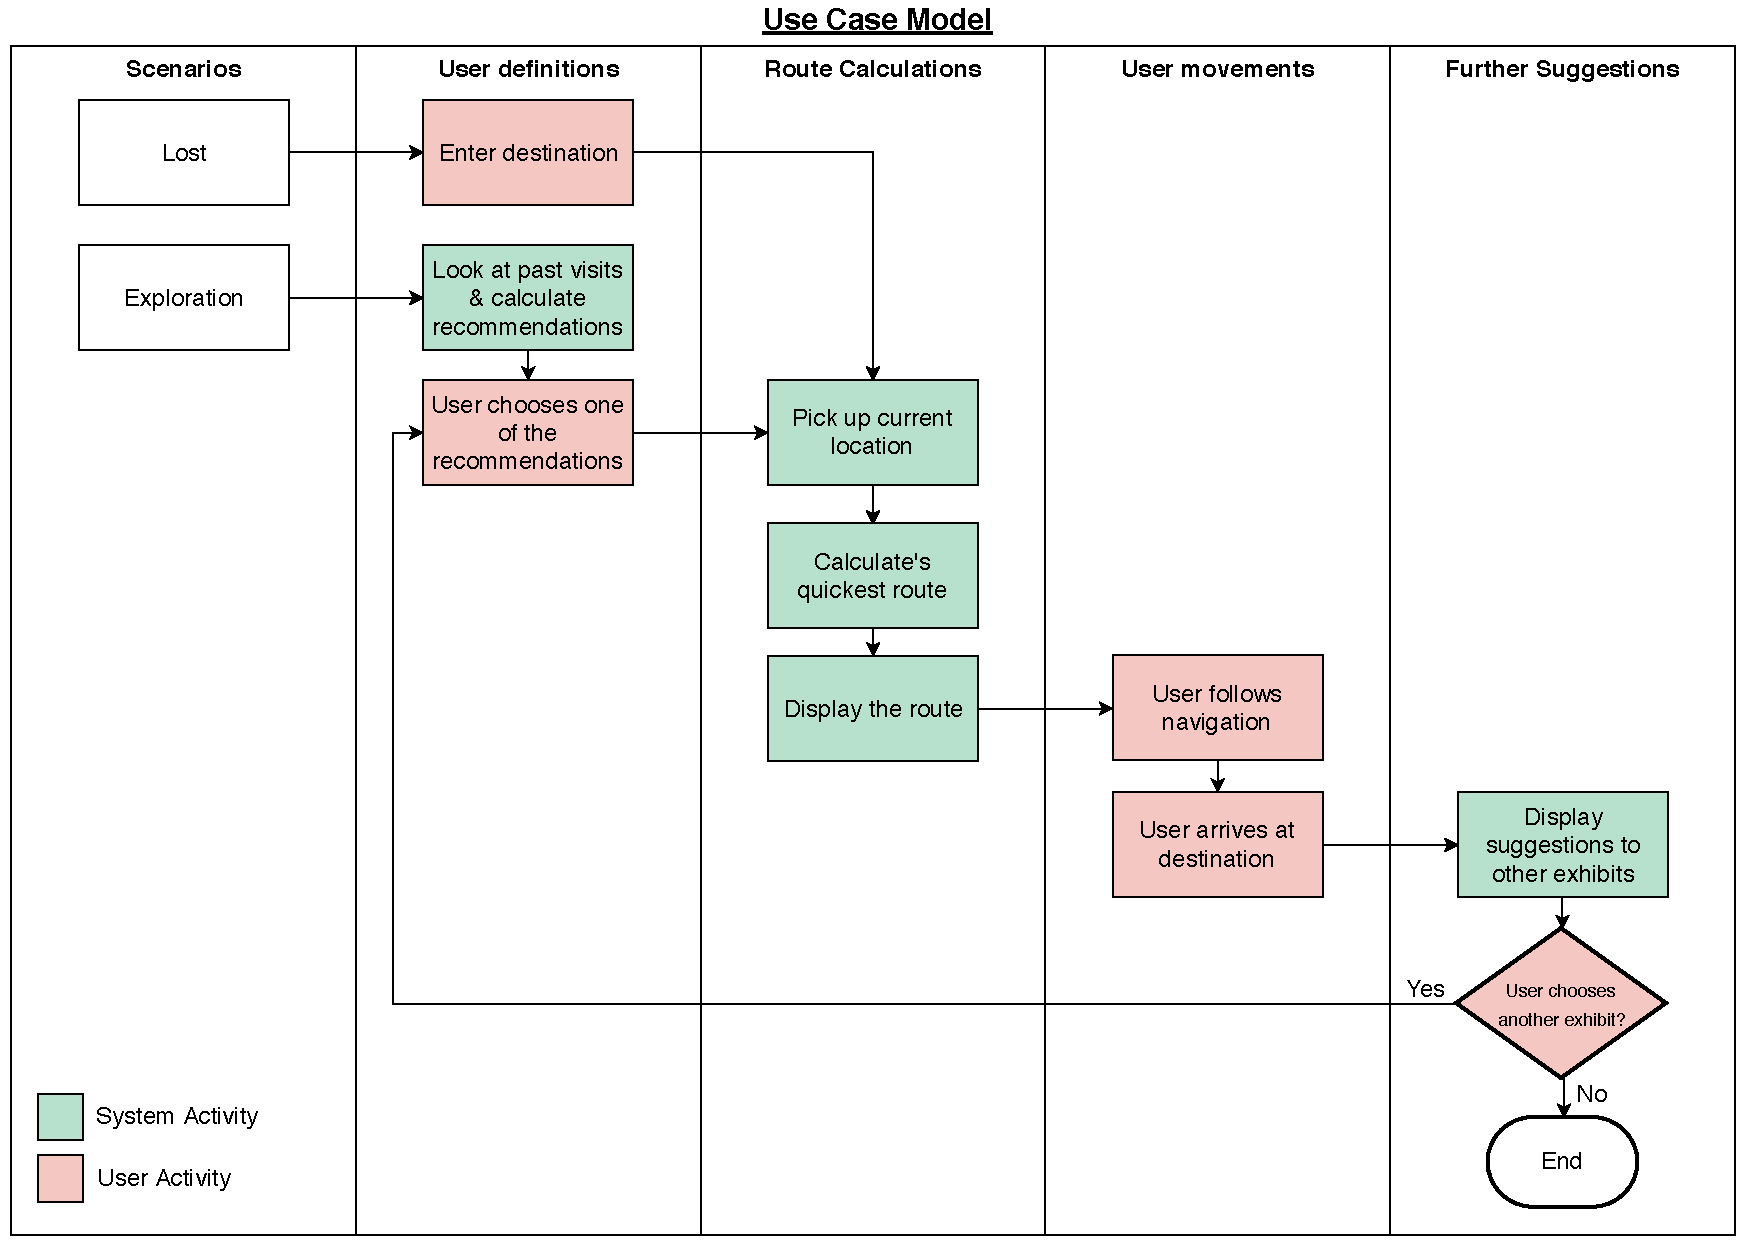
\includegraphics[width=\textwidth]
    {uml/use_case.pdf}
    \caption{Use Case Diagram}
    \label{fig:Use Case Diagram}
\end{figure}

\subsection{Activity Model}
This is based on the back-end of the application for example when the user searches about the museum, this history saved in the server where if the user wants to go to the same place then they can use our function called past visit.

\begin{figure}[H]
    \centering
    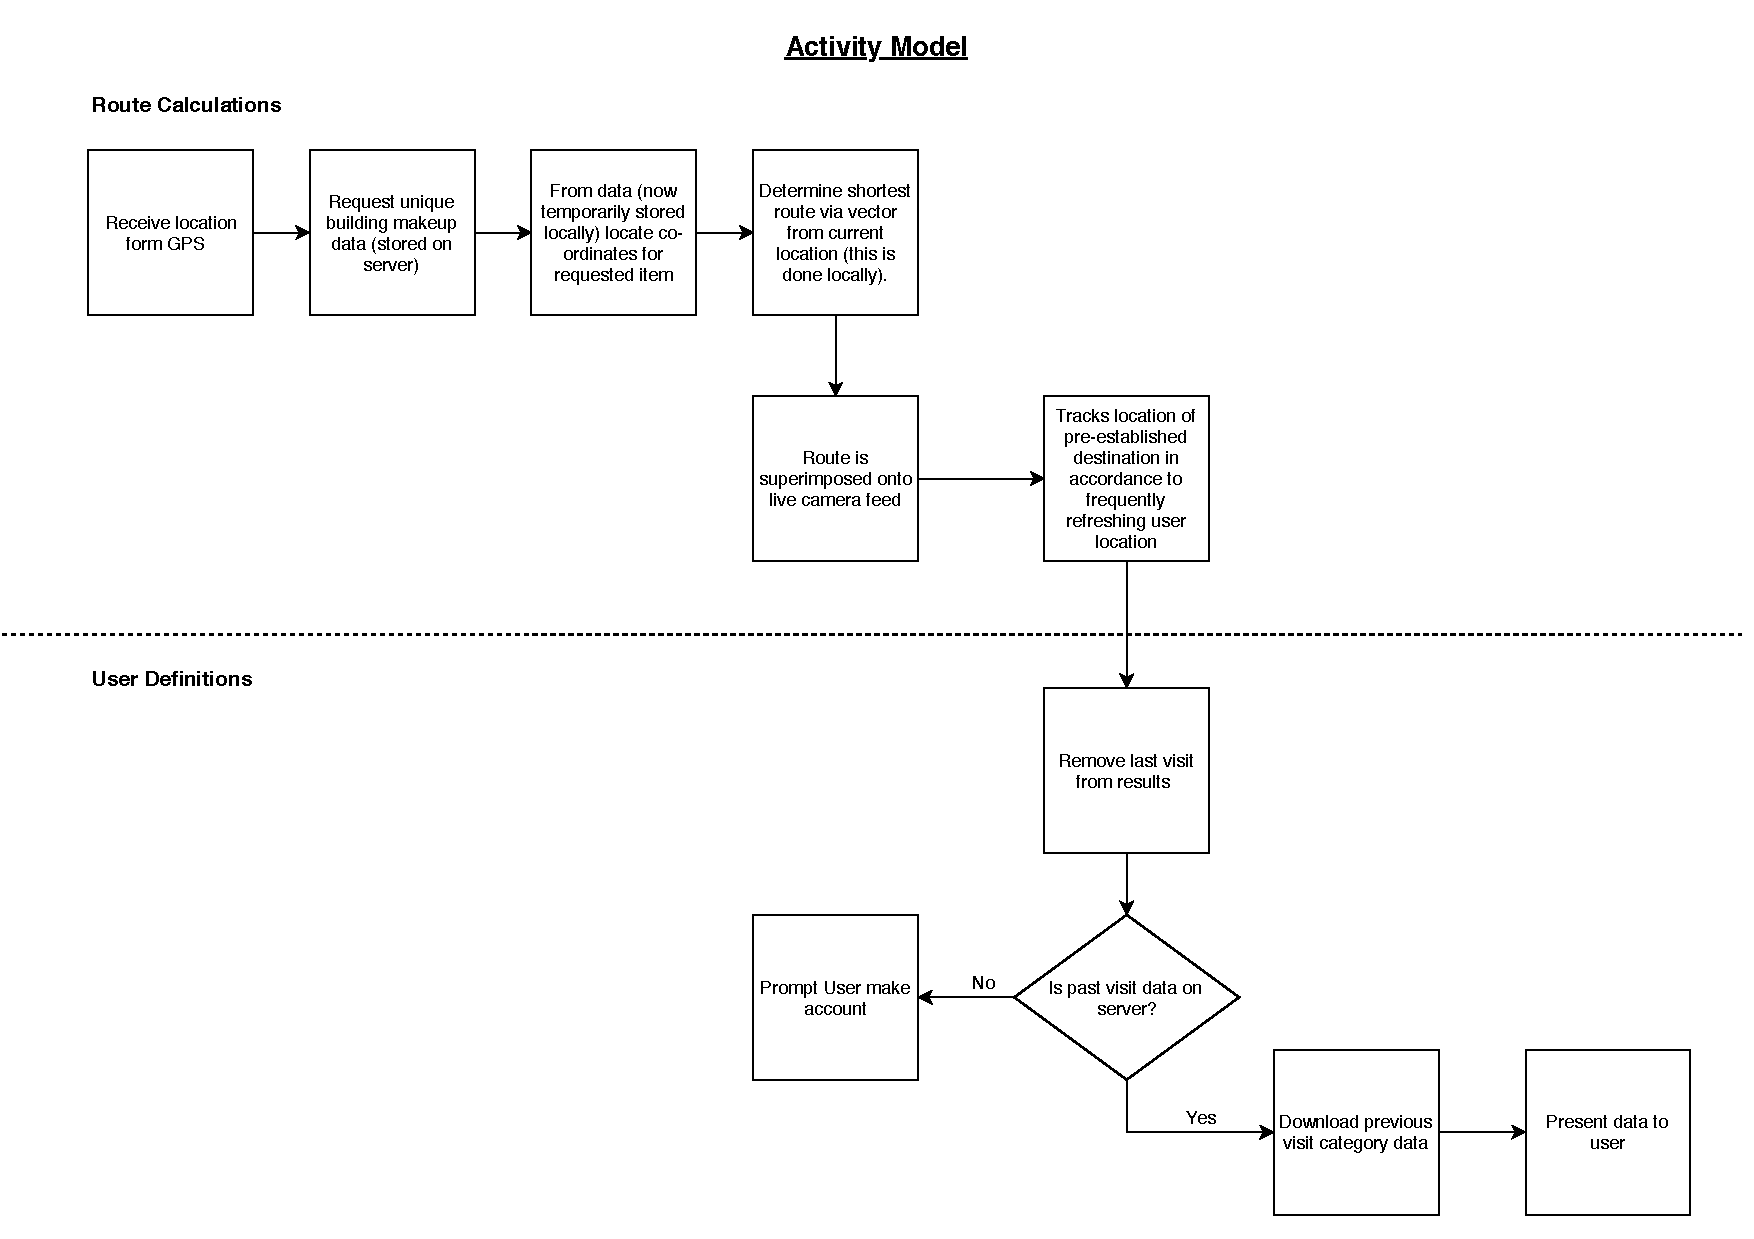
\includegraphics[angle=90, width=\textwidth]
    {uml/activity_diagram.pdf}
    \caption{Activity Model Diagram}
    \label{fig:Activity Model Diagram}
\end{figure}

\newpage
\subsection{User \& Acceptance Stories}
This will describe what will be achieved once the application is ready to be used by the user. A diagram has been created based on different scenarios where it can be found if the application has achieved the user needs. 

\begin{figure}[H]
    \centering
    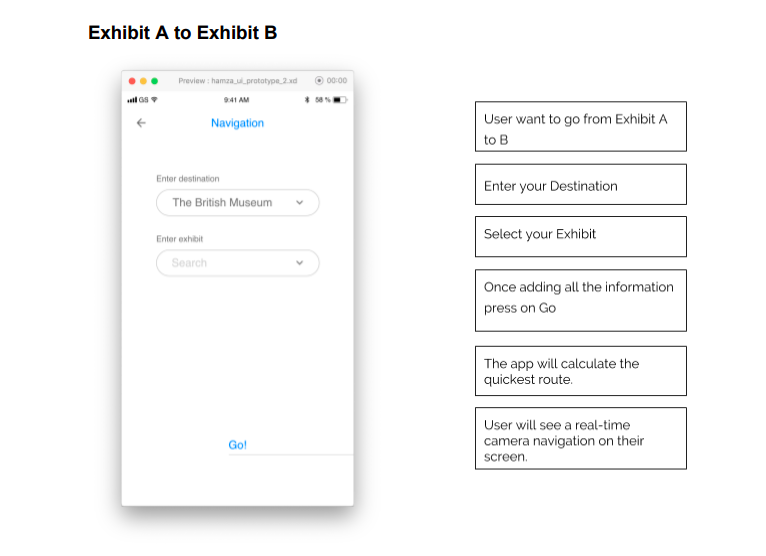
\includegraphics[width=\textwidth]
    {userstories/userstory_aTob.png}
    \caption{Going from point A to point B}
    \label{fig:AtoB}
\end{figure}

\begin{figure}[H]
    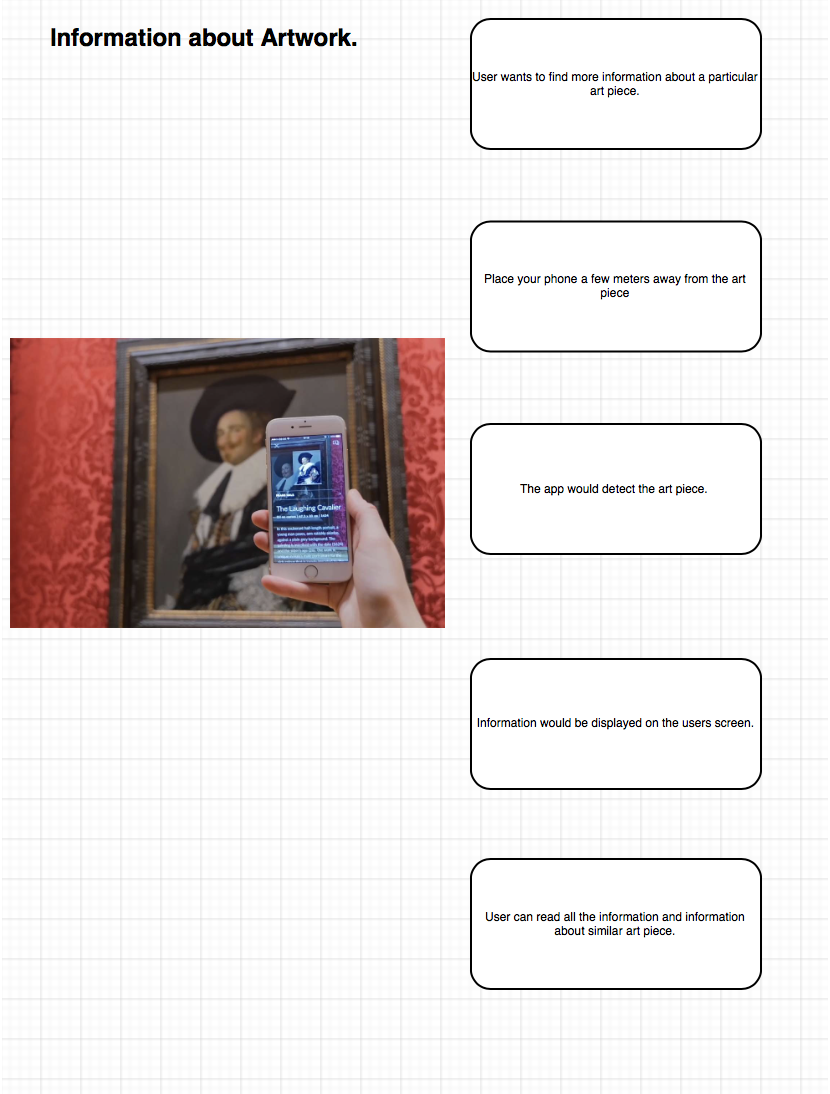
\includegraphics[width=\textwidth]
    {userstories/userstory_info.png}
    \caption{Getting information from exhibition}
    \label{fig:infofromexhibit}
\end{figure}

\begin{figure}[H]
    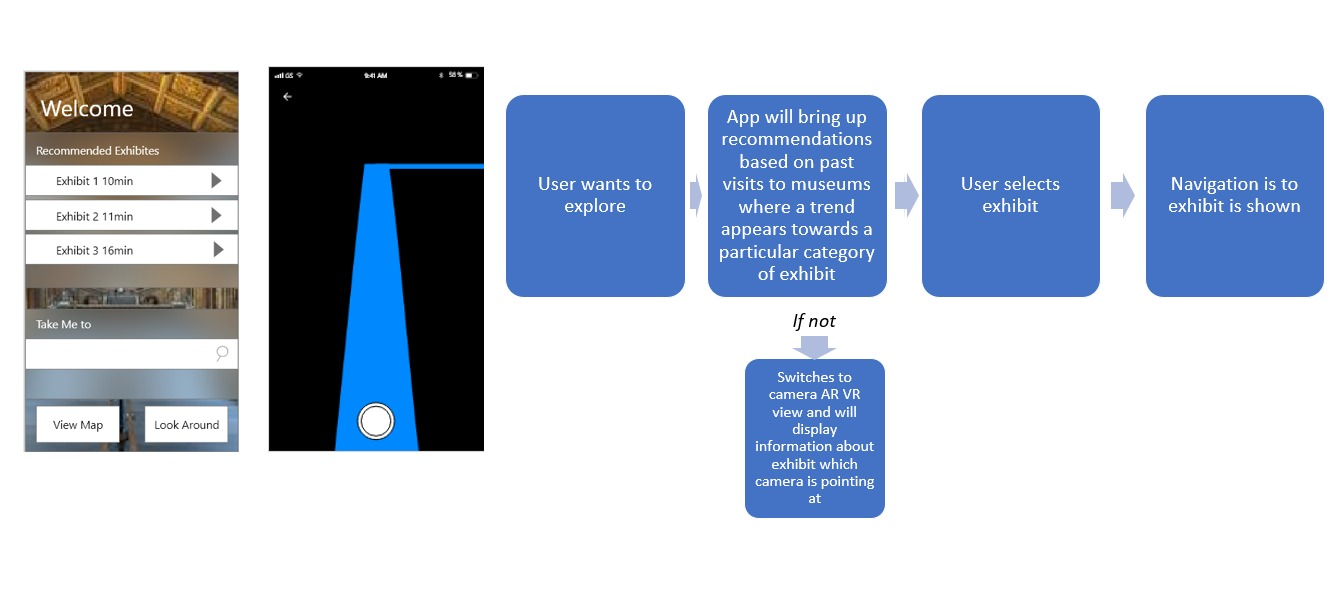
\includegraphics[width=\textwidth]
    {userstories/userstory_explore.jpeg}
    \caption{Exploring the museum}
    \label{fig:exploring}
\end{figure}

\section{Functional Requirements}
\begin{enumerate}
    \item Needs to be able to navigate the user from point A to B.
    \item The system should be able to display navigational routes in real-time.
    \item It should be able to calculate the quickest route.
    \item A 3D line should be superimposed through augmented reality to display the navigation to the user's destination.
    \item Camera recognition on artwork/exhibits, displaying further information about the exhibit.
    \item When user arrives at destination, the system should give a recommendation based on their route.
\end{enumerate}

\section{Non-functional Requirements}
\begin{enumerate}
    \item \textbf{Performance}: The system should respond quickly to user input, e.g user wants to find more information about an art piece or whenever they search up a location. The system should not require extensive CPU usage, it should not slow the device down inconveniencing the user.
    \item \textbf{Usability}: The system should have a simple layout, with appropriate colour used in appropriate contexts. The language used on the app should be easy to understand for the users. Having done research based on the user preference, it was discovered that users dislike too much text on their menu screen.
    \item \textbf{Data Usage}: Data usage should be kept to a minimum, only querying the relevant information (user location and exhibit information). Also, the app would require internet connection in order to calculate the real-time distance of the final destination from the user's current location.
    \item \textbf{Safety}: The system needs to have the ability to detect immutable objects obstructing the user's path. This can reduce common user accidents when using a mobile phone whilst walking.
    \item \textbf{Security}: Ensuring that the device's current location cannot be obtained by unauthorised third-party users is crucial in ensuing the security of using the platform.
\end{enumerate}
    
}